\documentclass[11pt]{article}
\usepackage[utf8]{inputenc}  % To control and create table of content
\usepackage{fancyhdr} 	% To create header
\usepackage{dirtytalk} % To create citations
\usepackage{array} % To control and create fixed size tables
\usepackage{longtable}
\usepackage{graphicx}
\graphicspath{ {Illustrationer/} }

\pagestyle{fancy}
\fancyhf{}
\lhead{Kravspecifikation}
\rhead{Version 0.1}
\rfoot{Page \thepage}

\renewcommand*\contentsname{Indholdsfortegnelse}

\begin{document}
	\begin{titlepage}
		\begin{center}
			\Large\textbf{Kravspecifikation}\\
			\large\textit{Version: 0.1}
		\end{center}
	\end{titlepage}
	
	\tableofcontents
	\newpage
	
	\section{Introduktion og baggrund}
	Formålet med dette dokument er at beskrive funktionelle og ikke-funktionelle krav for per konditionerings blodtryks apparatet. De funktionelle krav vil blive beskrevet ved hjælp af fully dressed use case diagrammer. 
	
	Beskrivelse af projektet: 
	
	\say{\textit{Akut blodprop i hjernen (Acute Ischemic Stroke – AIS) er en førende årsag til død og alvorlig handicap hos personer over 60 år.Intravenøs trombolysebehandling administreret indenfor 4,5 time fra symptomdebut er den nuværende bedste medicinske behandling. Grundet sikkerhedshensyn og det snævre tidsvindue er det desværre kun et fåtal af AIS patienterne, der modtager denne behandling. Målet er at opløse blodproppen og genoprette blodforsyning og dermed redde hjernevæv, der lider af iltmangel men endnu ikke er dødt. Om et område af hjernen dør eller står til at redde ved en blodprop afhænger ikke kun af selve blodproppen men også om hjernen er i stand til at få blod via omveje dannet af hjernens små blodkar. Et område af hjernen går til grunde med det samme (infarktkernen). Denne kerne af dødt hjernevæv kan i dagene efter en blodprop sprede sig og vokse. Der er således behov for at kunne beskytte hjernen mod iltmangel og øge andelen af hjernevæv, der overlever en blodprop. Iltmangel induceret periodevis i et fjernt organ (remote ischemic conditioning RIC) kan udføres ved at puste en blodtryksmanchet med afklemning af armen. Konditionering kan leveres som pre, per, og postconditionering, afhængig af om stimulus udøves før iltmangel, under iltmangel men før blodproppen er opløst og endelig efter blodproppen er opløst. Dyrestudier og senest kliniske studier har vist at RIC kan mindske det område af hjertet eller hjernen, der dør ved en blodprop. Det er ikke tilstrækkeligt undersøgt om RIC mindsker risikoen for handicap efter en blodprop i hjernen.}}
	
	\section{System beskrivelse}
	System er beregnet til behandling af patienter med \textit{acute ischemic stroke(AIS)}. Formålet er pre, per og postkonditioning af disse patienter. Systemet skal kunne lave arteriel okklusion i de øverste ydre ekstremiteter. For at sikre tilstrækkelig okklusion, skal det systoliske blodtryk først måles og derefter pumpe cuffen op til plus 25 mmHg over det målet tryk. Som minimum skal der afklemmes med et tryk på 180 mmHg. Okklusionen bliver holdt konstant i 5 minutter, hvor efter trykket lukkes ud der holdes en "pause" på 5 minutter. Denne process gentages ind til konditioneringen er færdig. 

	\section{Funktionelle krav}
	
	%Aktør beskrivelse
		\section{Aktør beskrivelse}
	Systemet har tre aktør og disse er beskrevet nedenfor. Aktørerne skal ses som brugere eller spillere der skal interagere med scenarierne for at de lykkes. 
	
	\begin{center}
		\begin{tabular}{ | m{4cm} | m{8cm}| } 
			\hline
			Aktørnavn& Medicinsk personale  \\ 
			\hline
			Aktørtype & Primær og sekundær \\ 
			\hline
			Beskrivelse af aktør & Aktør som påmontere manchetten og styre konditionering eller person som observere de gemte data fra behandlingsforløb\\ 
			\hline
		\end{tabular}
	\end{center}
	
	\begin{center}
		\begin{tabular}{ | m{4cm} | m{8cm}| } 
			\hline
			Aktørnavn& Patient \\ 
			\hline
			Aktørtype & Sekundær \\ 
			\hline
			Beskrivelse af aktør & En person med AIS som skal konditioneres\\ 
			\hline
		\end{tabular}
	\end{center}
	
	\begin{center}
		\begin{tabular}{ | m{4cm} | m{8cm}| } 
			\hline
			Aktørnavn& Database \\ 
			\hline
			Aktørtype & Sekundær \\ 
			\hline
			Beskrivelse af aktør & Gemmer data og logfiler omkring konditionerings forløb\\ 
			\hline
		\end{tabular}
	\end{center}
	
	\begin{center}
		\begin{tabular}{ | m{4cm} | m{8cm}| } 
			\hline
			Aktørnavn& Bruger \\ 
			\hline
			Aktørtype & Primær \\ 
			\hline
			Beskrivelse af aktør & Person der gør brug af konditioneringsapparatet til okklusionstræning, denne person behøver ikke besidde særlig faglig viden \\ 
			\hline
		\end{tabular}
	\end{center}
	\pagebreak
	
	%Use case 1
	\subsection{Use case 1 - Konditionering}
\begin{center}
		\begin{longtable}{ | p{0.3\textwidth} | p{0.7\textwidth}| } 
			\hline
			Goal& Gennemføre konditioneringsbehandling  \\ 
			\hline
			Initiation &  Medicinsk personale\\
			\hline
			Actors and stakeholders & 
			\begin{itemize}
				\item Medicinsk personale(primær)
				\item Patient (sekundær)
			\end{itemize} \\ 
			\hline
			References & Use case 3 \\ 
			\hline
			Number of concurrent occurrences & En til mange\\ 
			\hline	
			Precondition & 
			\begin{itemize}
				\item Mode switch er sat til “\textit{Konditionering}”
			\end{itemize} \\ 
			\hline
			Postcondition & 
			\begin{itemize}
				\item 5 hele cyklus er gennemført og gemt på hukommelsen
			\end{itemize} \\ 
			\hline
			Main scenario & \begin{enumerate}
				\setlength\itemsep{0cm} % Decrease line distance
				\item \textit{Medicinsk personale} placerer manchetten på patienten
				\item Knappen [Start/Stop] trykkes
				\item Et nyt patient ID genereres
				\subitem[Extension \#1] 
				\item Patient ID’et vises på skærmen
				\item Blodtrykket måles via \textit{use case 3}
				\subitem[Extension \#2]
				\item Blodtrykket vises på displayet og værdien gemmes i hukommelse
				\item Cuffen fyldes med luft til et tryk på 25 mmHG over systolisk tryk (minimum 180 mmHg)
			\end{enumerate} \\ 
			\hline
			Main scenario & \begin{enumerate}
				\setlength\itemsep{0cm} % Decrease line distance
				\setcounter{enumi}{7}				
				\item Tidsstempel gemmes når trykket er opnået
				\item Trykket opretholdes i 5 minutter(Okklusion) og resterende tid vises på displayet
				\item Blodtrykket måles via \textit{use case 3}
				fra punkt 2.
				\item Deflaterer cuffen helt og forbliver i dette stadie i 5 min(Reperfusion) Ved deflation start gemmes tidsstempel. Tid til næste okklusion vises på displayet
				\item Gentag punkt 7-11 (en cyklus) fire gange. Det nuværende cyklus nummer vises i displayet
			\end{enumerate} \\ 
			\hline
			Extensions & [Extension \#1] Et patient ID eksisterer allerede på apparatet. Der genereres ikke noget nyt patient ID.
			
			[Extension \#2] Blodtrykket kunne ikke måles. Gentag use case 3 hvis extension 2 ikke lige er eksekveret. Ellers skrives i display “FEJL kunne ikke måle blodtryk” og use casen stopper    .  \\
			\hline
		\end{longtable}
		
	\end{center}
	\pagebreak
	
	%Use case 2
		\subsection{Use case 2 - Initialiser blodtryksmåling }
	\begin{table}[H]
		\begin{center}
			\begin{tabular}{ | p{0.24\textwidth} | p{0.7\textwidth}| } 
				\hline
				Mål& Mål et blodtryk\\ 
				\hline
				Initiering &  Medicinsk personale\\
				\hline
				Aktører og interessenter & 
				\begin{itemize}
					\item Medicinsk personale(primær)
					\item Patient (sekundær)
				\end{itemize} \\ 
				\hline
				Referencer & Mål blodtryk(UC3) \\ 
				\hline
				Antal samtlige forekomster & En til mange\\ 
				\hline	
				Startbetingelser & 
				\begin{itemize}
					\item Manchetten er placeret på armen
					\item Mode switch er sat til “\textit{Konditionering}”
				\end{itemize} \\ 
				\hline
				Slutbetingelser & 
				\begin{itemize}
					\item Patientens blodtryk er målt
				\end{itemize} \\ 
				\hline
				Normal forløb & \begin{enumerate}
					\setlength\itemsep{0cm} % Decrease line distance
					\item Brugeren trykker på [Mål blodtryk]
					\item Et nyt patient ID genereres
					\subitem [Undtagelse \#1] 
					\item Patient ID’et vises på skærmen
					\item Blodtrykket måles via \textit{use case 3}
					\subitem [Undtagelse \#2]
				\end{enumerate} \\ 
				\hline
				Undtagelser &  [Undtagelse \#1] Et patient ID eksisterer allerede på apparatet. Der genereres ikke noget nyt patient ID.
				
				[Undtagelse \#2] Blodtrykket kunne ikke måles. Gentag use case 3 hvis undtagelse 2 ikke er blevet eksekveret inden for 2 minutter. Ellers skrives i display “FEJL kunne ikke måle blodtryk” og use casen stopper\\ 
				\hline
				
			\end{tabular}
		\end{center}
		\caption{\textit{Fully dressed} use case diagram over use case 2}
			\end{table}
		\newpage
	
	%Use case 3
		\subsection{Use case 3 - Mål blodtryk}
	\begin{table}[H]
		\begin{center}
			\begin{tabular}{ | p{0.24\textwidth} | p{0.7\textwidth}| } 
				\hline
				Mål & Mål et systolisk, diastolisk og middel(MAP) tryk\\ 
				\hline
				Initiering &  Konditionering (UC1) eller Initialiser blodtryksmåling (UC2)\\
				\hline
				Aktører og interessenter & - \\
				\hline
				Referencer & - \\ 
				\hline
				Antal samtlige forekomster & En til mange\\ 
				\hline	
				Startbetingelser & 
				\begin{itemize}
					\item Patient ID er oprettet
					\item Manchetten er placeret på armen
					\item Mode switch er sat til “\textit{Konditionering}”
				\end{itemize} \\ 
				\hline
				Slutbetingelser & 
				\begin{itemize}
					\item Blodtrykket er mål
				\end{itemize} \\ 
				\hline
				Normal forløb & \begin{enumerate}
					\setlength\itemsep{0cm} % Decrease line distance
					\item Manchetten fyldes til tryk over systolisk niveau 
					\item Luften lukkes gradvist ud og det systoliske tryk registreres 
					\item Middel trykket (MAP) måles 
					\item Det diastoliske tryk udregnes ud fra systole og MAP 
					\item Blodtrykket vises på skærmen og værdien gemmes i hukommelsen med et tidsstempel 
				\end{enumerate} \\ 
				\hline
				Undtagelser & -\\ 
				\hline
			\end{tabular}
		\end{center}
			\caption{\textit{Fully dressed} use case diagram over use case 3}
			\end{table}
			\newpage
	
	%Use case 4
		\subsection{Use case 4 - Overfør data}
	\begin{table}[H]
		\begin{center}
			\begin{tabular}{ | p{0.24\textwidth} | p{0.7\textwidth}| } 
				\hline
				Mål & Eksportér data fra blodtryksapparat til databasen\\ 
				\hline
				Initiering &  Medicinsk personale\\
				\hline
				Aktører og interessenter & 
				\begin{itemize}
					\item Medicinsk personale(primær)
					\item Patient (sekundær)
				\end{itemize} \\ 
				\hline
				Referencer & - \\ 
				\hline
				Antal samtlige forekomster & Én pr behandlingsforløb \\ 
				\hline	
				Startbetingelser & 
				\begin{itemize}
					\item Der eksisterer en logfil på hukommelsen
				\end{itemize} \\ 
				\hline
				Slutbetingelser & 
				\begin{itemize}
					\item Logfilen er overført til database
					\item Blodtryksapparat udstyres med formateret hukommelse og klar til næste patient
				\end{itemize} \\ 
				\hline
				Normal forløb & \begin{enumerate}
					\setlength\itemsep{0cm} % Decrease line distance
					\item Tag SD kortet ud af blodtryksapparatet 
					\item Sæt SD kortet i computeren og overfør filen 
					\item Formatér SD kortet
					\item Sæt SD kortet tilbage i konditioneringsapparatet 
				\end{enumerate} \\ 
				\hline
				Undtagelser & -\\ 
				\hline
			\end{tabular}
		\end{center}
		
			\caption{\textit{Fully dressed} use case diagram over use case 4}
		\end{table}
			\newpage
	
	%UseCase 5
		\subsection{Use case 5 - Sikkerhedskontrol med pulsoximeter}
		\begin{center}
			\begin{tabular}{ | p{0.3\textwidth} | p{0.7\textwidth}| } 
				\hline
				Mål & Sikre at patientens kredsløb tåler konditionering \\ 
				\hline
				Initiering &  Konditionering (UC1)\\
				\hline
				Aktører og interessenter & 
				\begin{itemize}
					\item Patient (sekundær)
				\end{itemize} \\ 
				\hline
				Referencer & - \\ 
				\hline
				Antal samtlige forekomster & En til mange \\ 
				\hline	
				Startbetingelser & 
				\begin{itemize}
					\item Konditionering (UC1) igangværende
					\item Pulsoximeteret er monteret på patients finger
					\item Patient har gennemført én afklemnings cyklus
 				\end{itemize} \\ 
				\hline
				Slutbetingelser & 
				\begin{itemize}
					\item Patients tilstand er bestemt 
				\end{itemize} \\ 
				\hline
				Normal forløb & \begin{enumerate}
					\setlength\itemsep{0cm} % Decrease line distance
					\item Saturation detekteres
					\item Saturation gemmes på SD-kort
					\item Saturation er tilfredsstillende
					\subitem [Undtagelse \#1.1][Undtagelse \#1.2]
					\item Behandlingen kan fortsætte
				\end{enumerate} \\ 
				\hline
				Undtagelser &  [Undtagelse \#1.1] Tegn på dårlig kredsløb: Blodtryksapparatet stopper konditionerings forløbet 
				[Undtagelse \#1.2] Kør use case 7\\ 
				\hline
			\end{tabular}
		\end{center}
			\pagebreak
	
	%UseCase 6
		\subsection{Use case 6 - Okklusionstræning}
		\begin{center}
			\begin{tabular}{ | p{0.3\textwidth} | p{0.7\textwidth}| } 
				\hline
				Goal& Gennemføre okklusion af venøs kredsløb under træning  \\ 
				\hline
				Initiation &  Bruger\\
				\hline
				Actors and stakeholders & 
				\begin{itemize}
					\item Bruger (primær)
				\end{itemize} \\ 
				\hline
				References & - \\ 
				\hline
				Number of concurrent occurrences & En pr træningspas \\ 
				\hline	
				Precondition & 
				\begin{itemize}
					\item Mode switch er sat til  “\textit{okklusionstræning}”
 				\end{itemize} \\ 
				\hline
				Postcondition & 
				\begin{itemize}
					\item Okklusions træningssæt gennemført
				\end{itemize} \\ 
				\hline
				Main scenario & \begin{enumerate}
					\setlength\itemsep{0cm} % Decrease line distance
					\item Montere manchetten på arm/ben
					\item Tryk på knap [Start/Stop]
					\item Manchetten pumpes op til 100mmHg
					\item Træningssættet begyndes og trykkes holdes konstant på 100mmHg (+/-10mmHg)
					\item Tryk på knap [Stop]
					\item Manchetten deflateres
				\end{enumerate} \\ 
				\hline
				Extensions & - \\ 
				\hline
			\end{tabular}
		\end{center}
	\pagebreak
		
	
	%UseCase 7
		\subsection{Use case 7 - Afbryd}
	\begin{table}[H]
			\begin{center}
			\begin{tabular}{ | p{0.3\textwidth} | p{0.7\textwidth}| } 
				\hline
				Mål & Tømme manchetten for luft og afbryde nuværende procedure \\ 
				\hline
				Initiering &  Medicinsk personale, Patient\\
				\hline
				Aktører og interessenter & 
				\begin{itemize}
					\item Medicinsk personale 
					\item Bruger 
				\end{itemize} \\ 
				\hline
				Referencer & Konditionering (UC1) og Mål blodtryk (UC3) \\ 
				\hline
				Antal samtlige forekomster & En til mange \\ 
				\hline	
				Startbetingelser & 
				\begin{itemize}
					\item Konditionering (UC1) og Mål blodtryk (UC3) er igangværende 
 				\end{itemize} \\ 
				\hline
				Slutbetingelser & 
				\begin{itemize}
					\item Behandlingen er afbrudt og manchetten er tom for luft
				\end{itemize} \\ 
				\hline
				Normal forløb & \begin{enumerate}
					\setlength\itemsep{0cm} % Decrease line distance
					\item Brugeren trykker på knappen [Start/Stop konditionering]
					\item Den igangværende use case afbrydes
					\item Manchetten tømmes for luft og tidsstempel med “\textit{Gennemført afklemning} = false” gemmes i hukommelsen
					\subitem[Undtagelse \#1]
				\end{enumerate} \\ 
				\hline
				Undtagelser & [Undtagelse \#1] Use case 6 er aktiv: ingen data gemmes i hukommelsen. \\ 
				\hline
			\end{tabular}
		\end{center}
			\caption{\textit{Fully dressed} use case diagram over use case 7}
		\end{table}
	\newpage

		
	
	%UseCase8
		\subsection{Use case 8 - Setup}
		\begin{table}[H]
				\begin{center}
			\begin{tabular}{ | p{0.24\textwidth} | p{0.7\textwidth}| } 
				\hline
				Mål & Ændre konditioneringsforholdene \\ 
				\hline
				Initiation &  Medicinsk personale\\
				\hline
				Aktører og interessenter & 
				\begin{itemize}
					\item Medicinsk personale 
				\end{itemize} \\ 
				\hline
				Referencer & Illustration over setup \\ 
				\hline
				Antal samtlige forekomster & En til mange \\ 
				\hline	
				Startbetingelser & 
				\begin{itemize}
					\item Mode switch er sat til “\textit{setup}” 
					\item Displayet er ændret til setup
 				\end{itemize} \\ 
				\hline
				Slutbetinglser & 
				\begin{itemize}
					\item Cyklus længden og/eller antallet er cyklusser er ændret
				\end{itemize} \\ 
				\hline
				Normal forløb & \begin{enumerate}
					\setlength\itemsep{0cm} % Decrease line distance
					\item Brugeren trykker på knappen [Mål blodtryk]  for at vælge \textit{Tid pr cyklus}
					\item Bruger trykker på knappen [Start/Stop] for at ændre \textit{Tid pr cyklus}
					\item Bruger trykker på knappen [Mål blodtryk]  for at gemme ændringen
					\item Bruger trykker på knappen [Start/Stop] for at navigere til \textit{Antal cyklusser}
					\item Ved knap tryk på [Mål blodtryk]  vælges \textit{Antal cyklusser}
					\item Ved knap tryk på [Start/Stop] ændre \textit{Antal cyklusser}
					\item Brugeren trykker på knappen [Mål blodtryk] for at gemme ændringen
				\end{enumerate} \\ 
				\hline
				Undtagelser & -  \\ 
				\hline
			\end{tabular}
		\end{center}

			\caption{\textit{Fully dressed} use case diagram over use case 8}
		\end{table}
			\newpage

	
	\section{Ikke-funktionelle krav }
	
	\subsection{Microcontroller}
	\begin{enumerate}
		\setlength\itemsep{0cm}
		\item Atmega32
		\end{enumerate}
	
	\subsection{Filformat og opsætning}
	\begin{enumerate}
		\setlength\itemsep{0cm} % Decrease line distance
		\item Data logged i formatet .csv og hver kolonne indeholder følgende værdier og enheder: 
		\begin{enumerate}
			\item Tidsstempel [yy:mm:dd hh:mm:ss]
			\item Afklemningstryk [mmHg]
			\item Gennemført afklemning [Boolean]
			\item Systoliske blodtryk [mmHg]
			\item Middelblodtryk (MAP) [mmHg]
			\item Diastolisk blodtryk [mmHg]
		\end{enumerate}
		\item Der oprettet én fil pr patient, med filnavn tilsvarende det unikke patient ID
	\end{enumerate}
	
	\subsection{Patient ID}
	\begin{enumerate}
		\setlength\itemsep{0cm} % Decrease line distance
		\item Består af karaktererne A-Z og tallene 0-9
		\begin{enumerate}
			\item ID’et er fem karakterer lang: ***** svarende til 60 millioner kombinationer
			\item ID’et er ikke case sensitiv
		\end{enumerate}
	\end{enumerate}
	
	
	\subsection{Hukommelse}
	\begin{enumerate}
		\setlength\itemsep{0cm} % Decrease line distance
		\item Information lagres på micro SDSC af typen:
		\begin{enumerate}
			\item Class 4
			\item Fil system [fat32] og minimum 128mb
		\end{enumerate}
	\end{enumerate}
	
	\subsection{Forsyning}
	\begin{enumerate}
		\setlength\itemsep{0cm} % Decrease line distance
		\item Konditionerings apparatet skal forsynes med 12V, min 2A
		\begin{enumerate}
			\item DC-connector (angiv diameter) 
			\item 8 stk AAA batterier (1,5V)
		\end{enumerate}
	\end{enumerate}
	
	%User interface 
	\section{User interface}
User interface består overordnede af en skærm og 2 knapper. En knap til at start og stoppe funktioner og en knap til at måle blodtryk. Til brugerfeedback er der en display hvorpå trykket, patient ID, resterende tid og antallet af gennemførte cyklusser vises. Apparatet betjenes i tre forskellige stadier “Konditionering, Okklusion og setup”. Disse tre stadier er beskrevet med hver siden illustration nedenfor. For at skifte mellem disse stadier er der en mode switch på bagsiden af apparatet, den er også beskrevet nedenfor: 

\subsection{Konditionering}
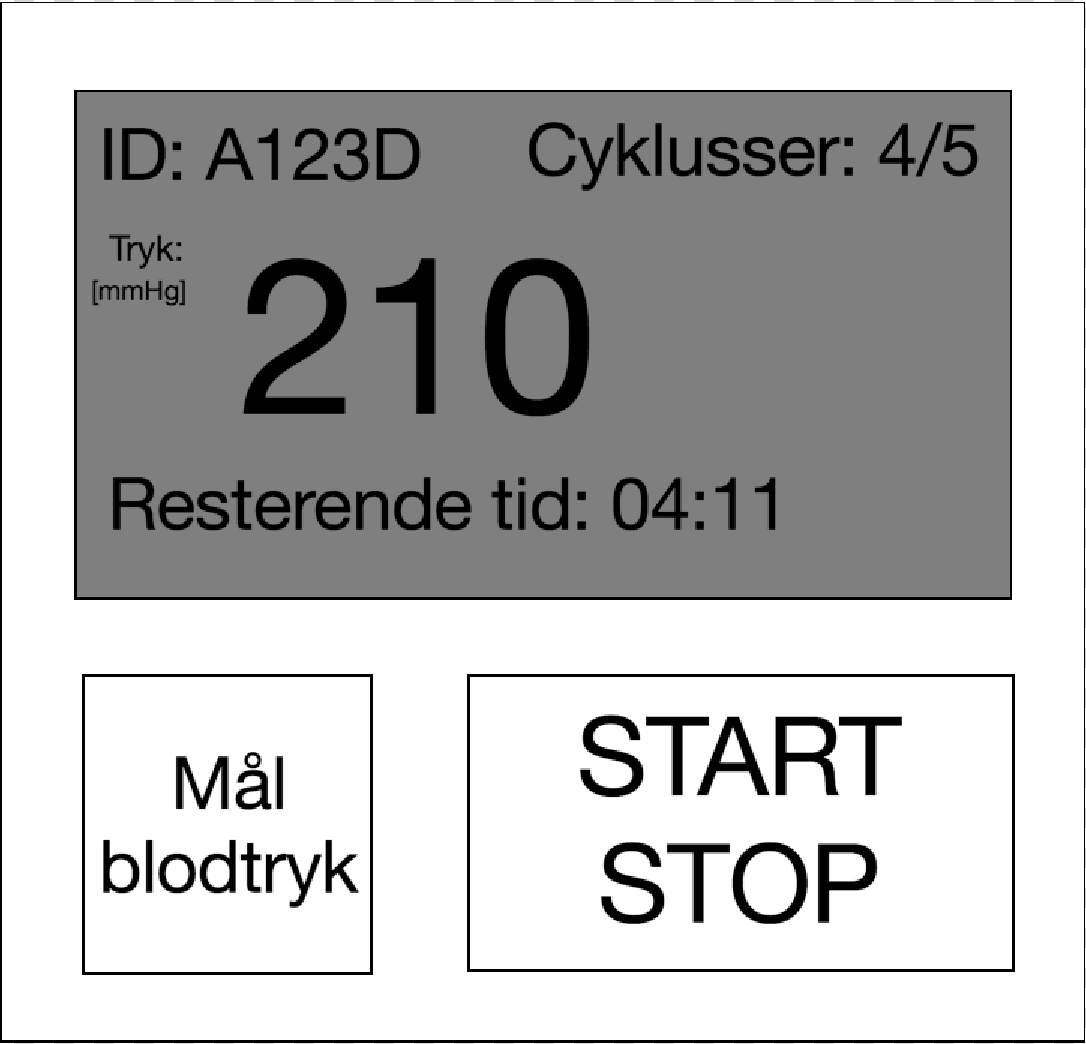
\includegraphics[width=\textwidth]{Illustrationer/KonditioneringGUI}
\subsection{Okklusion}
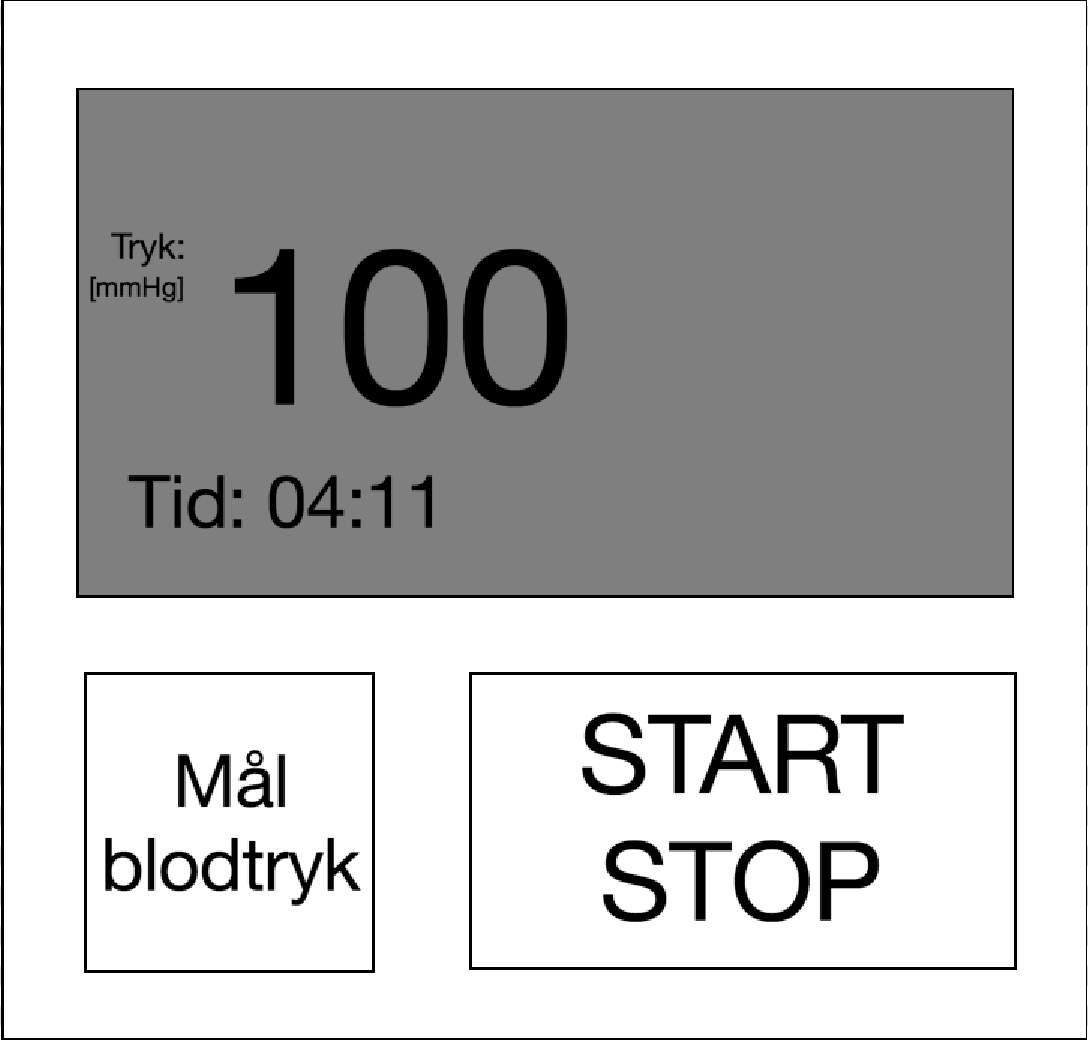
\includegraphics[width=\textwidth]{Illustrationer/OkklusionGUI}

\subsection{Setup}
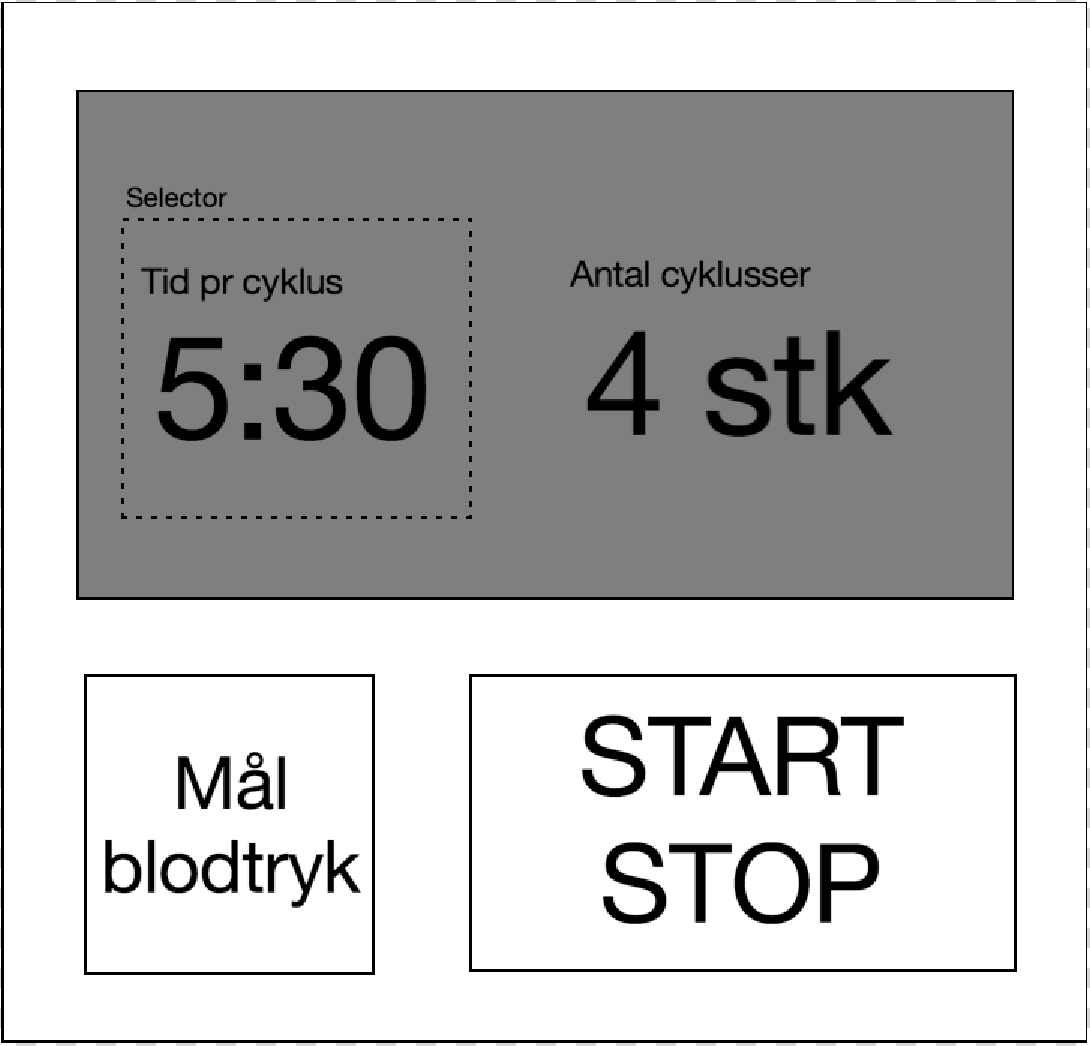
\includegraphics[width=\textwidth]{Illustrationer/SetupGUI}

\subsection{Bagside}
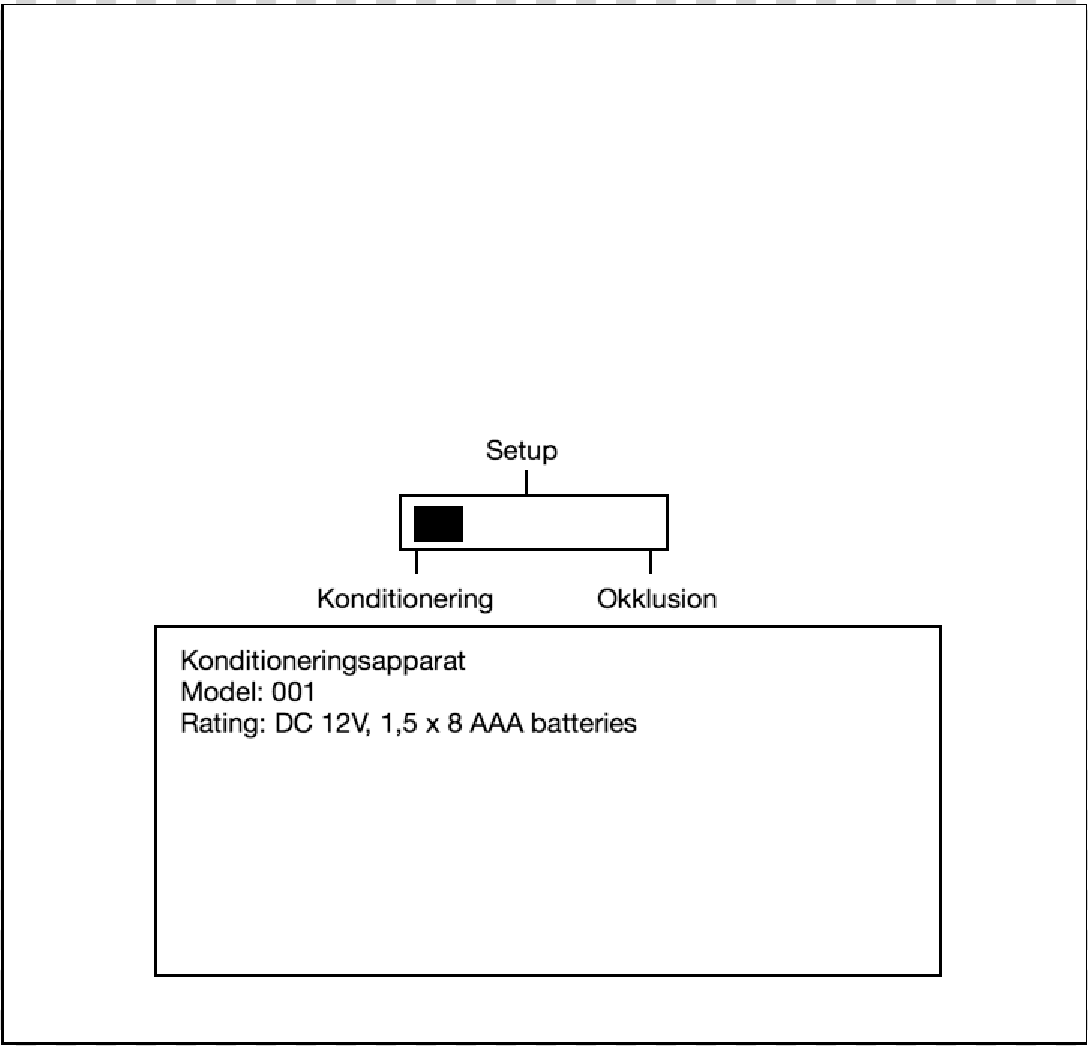
\includegraphics[width=\textwidth]{Illustrationer/BagsideGUI}

	
	
\end{document}